\chapter{Proces trenowania sieci neuronowych}
\thispagestyle{chapterBeginStyle}

\section{Opis procesu trenowania}

Trenowanie sieci neuronowej składa się z cyklicznych operacji, które mają za zadanie minimalizować funkcję kosztu. W każdym cyklu należy wybrać element zbioru treningowego, uzyskać predykcje modelu, obliczyć gradienty funkcji kosztu względem parametrów modelu oraz dokonać odpowiednich zmian w parametrach. Ważne jest monitorowanie zmian funkcji kosztu na zbiorze walidacyjnym (zbiór rozłączny z treningowym). Algorytm zmieniania parametrów sieci określony jest mianem optymalizatora. Poniżej opisany jest pseudokod algorytmu \texttt{train\_models}, który ma za zadanie przeprowadzić proces trenowania sieci neuronowych.

\section{Pseudokod algorytmu \texttt{train\_models}}

\begin{pseudokod}[H]
    \SetAlgoLined
    \DontPrintSemicolon
    \textbf{Dane wejściowe:} $nn\_architectures$\Comment*[r]{Lista zawierająca opisy architektur poszczególnych sieci neuronowych}
    
    \BlankLine
    $models \leftarrow \lbrack \rbrack$\;
    $train\_data\_loader \leftarrow init\_tr\_dl(batch=16)$\Comment*[r]{Obiekt zwracający podzbiory (mocy = 16) zbioru treningowego}
    $valid\_data\_loader \leftarrow init\_vl\_dl(batch=16)$\Comment*[r]{Obiekt zwracający podzbiory (mocy = 16) zbioru walidacyjnego}
    
    \BlankLine
    \For{$nn\_architecture$ $\in$ $nn\_architectures$}{
        $nn \leftarrow init\_nn(nn\_architecture)$\Comment*[r]{Inicjalizacja sieci zgodnie z opisem architektury}
        $models.append(nn)$\;
    }
    
    \BlankLine
    \Do{process\_not\_killed}{
        $tr\_batch \leftarrow train\_data\_loader.get\_batch()$\Comment*[r]{Pozyskanie 16 elementów zbioru treningowego}
        
        \BlankLine
        \For{$nn$ $\in$ $models$}{
            $pred\_y \leftarrow nn.predict(tr\_batch)$\Comment*[r]{Wykonanie 16 predykcji dla 16 elementów zbioru treningowego}
            $tr\_loss \leftarrow L(tr\_batch.y, pred\_y)$\Comment*[r]{Obliczenie średniej wartości funkcji kosztu dla 16 elementów}
            $grad \leftarrow get\_gradients(tr\_loss)$\Comment*[r]{Gradienty uśrednionej funkcji kosztu (na 16 elementach)}
            $nn.optimizer.update\_parameters(grad)$\Comment*[r]{Wykonanie aktualizacji parametrów przez optymalizator}
            
            \BlankLine
            \uIf{$mod(tr\_batch.num, 5000) == 0$\Comment*[r]{Co 5 tys. iteracji trenujących, wykonuje się walidację modelu}}{
                $vl\_loss\_list \leftarrow \lbrack \rbrack$\;
                \BlankLine
                
                \For{$vl\_batch$ $\in$ $valid\_data\_loader$}{
                $pred\_y \leftarrow nn.predict(vl\_batch)$\Comment*[r]{Wykonanie predykcji dla każdego podzbioru }
                $vl\_loss\_list.append(L(vl\_batch.y, pred\_y))$\Comment*[r]{Średnia wartość funkcji kosztu dla 16 elementów}
                }
                
                \BlankLine
                print(vl\_loss\_list.mean())\Comment*[r]{Wypisujemy średnią wartość funkcji kosztu na zbiorze walidacyjnym}
            }
        }
        \BlankLine
    }
    
    \caption{Algorytm train\_models}
\end{pseudokod}

\newpage

\section{Wizualizacja procesu trenowania}
\subsection{Z użyciem rasteryzatora \texttt{SemBoxRasterizer}}
\begin{figure}[h!]
    \centering
    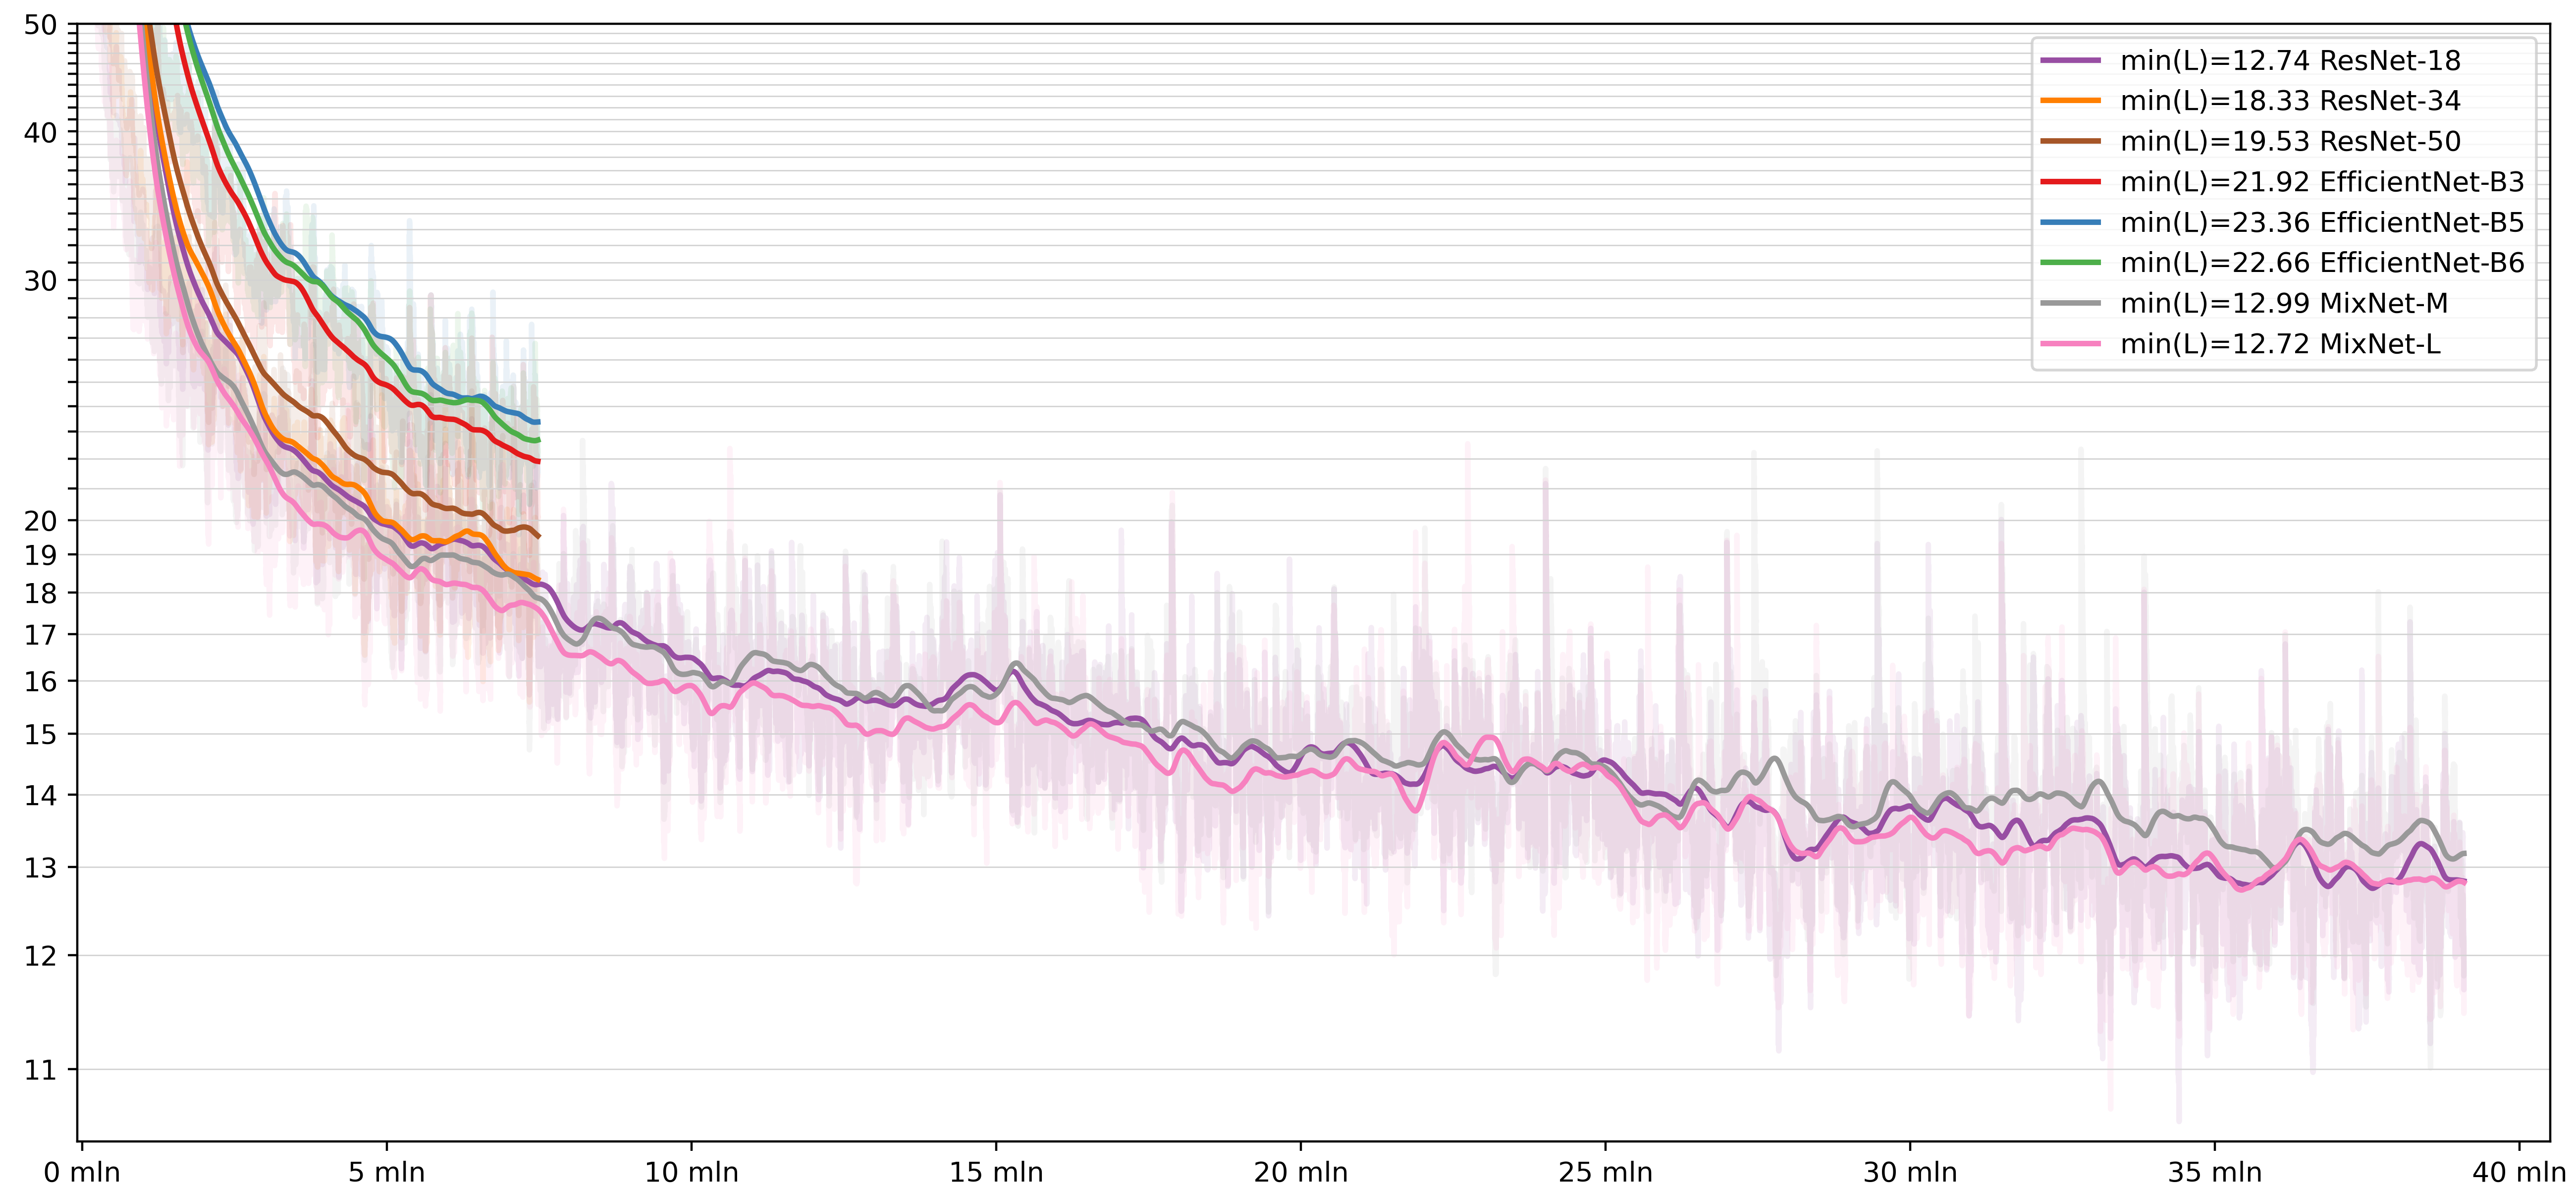
\includegraphics[width=\linewidth]{loss_sembox_train.png}
    \caption{Wartości funkcji $L$ dla próbek ze zbioru \textbf{treningowego} (wartości najmniejsze podane są dla krzywych uzyskanych z wygładzenia wykładniczego wartości funkcji $L$)}
    \vspace*{1cm}
    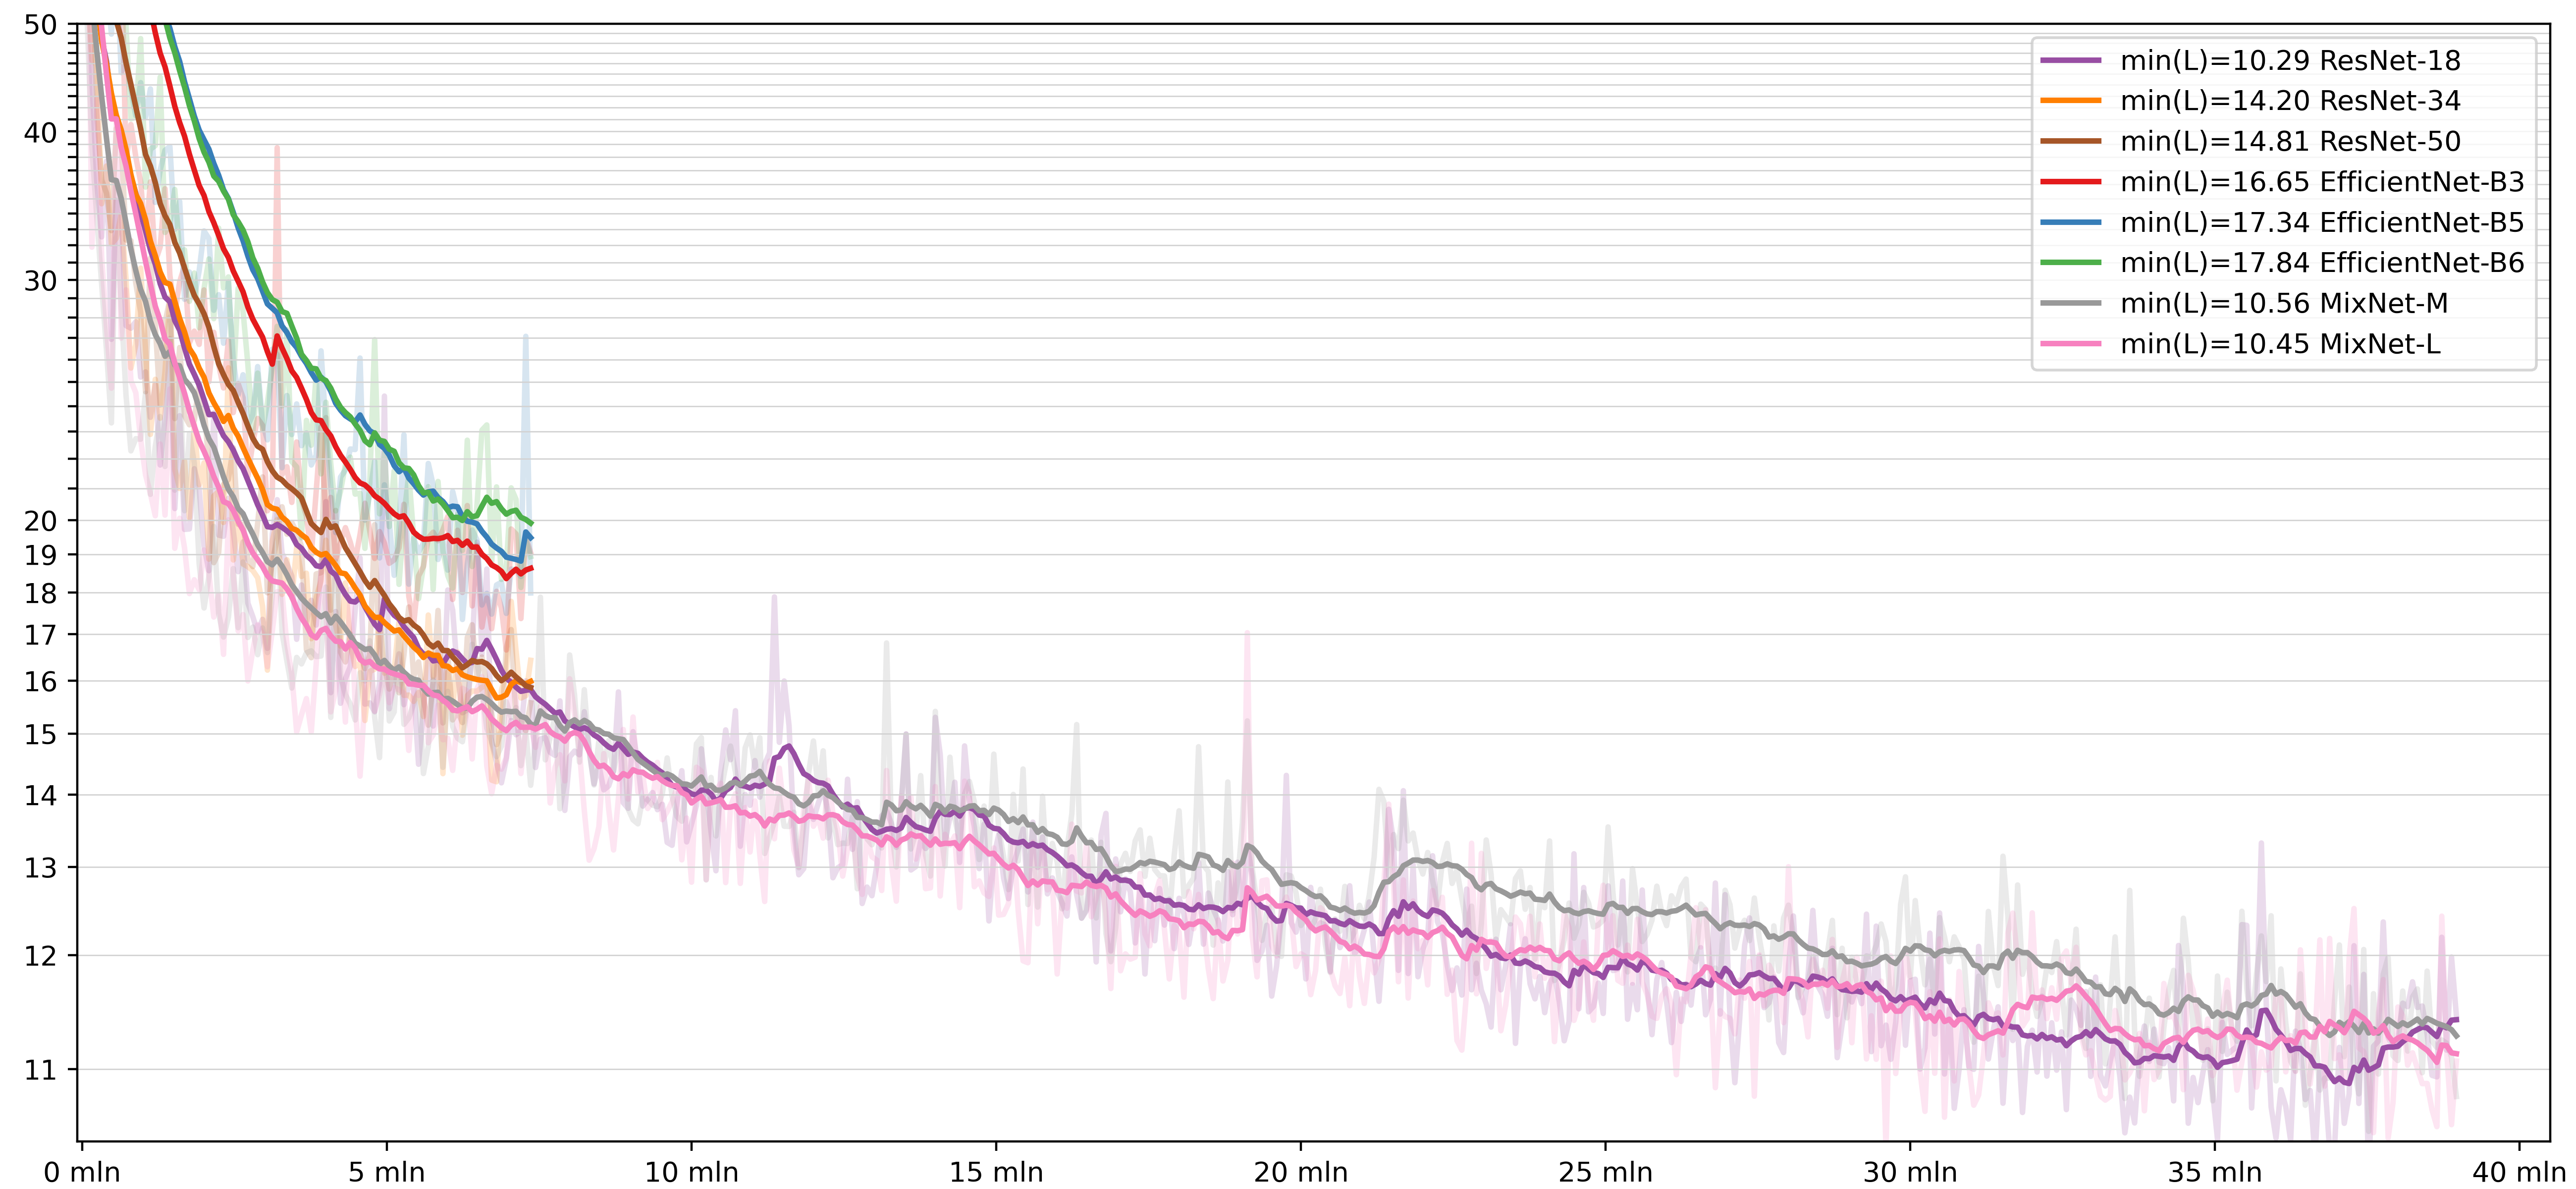
\includegraphics[width=\linewidth]{loss_sembox_val.png}
    \caption{Wartości funkcji $L$ dla próbek ze zbioru \textbf{walidacyjnego} (wartości najmniejsze podane są dla dokładnych wartości funkcji $L$)}
\end{figure}

\newpage

\subsection{Z użyciem rasteryzatora \texttt{CenterLines}}
\vspace*{0cm}

\begin{figure}[h!]
    \centering
    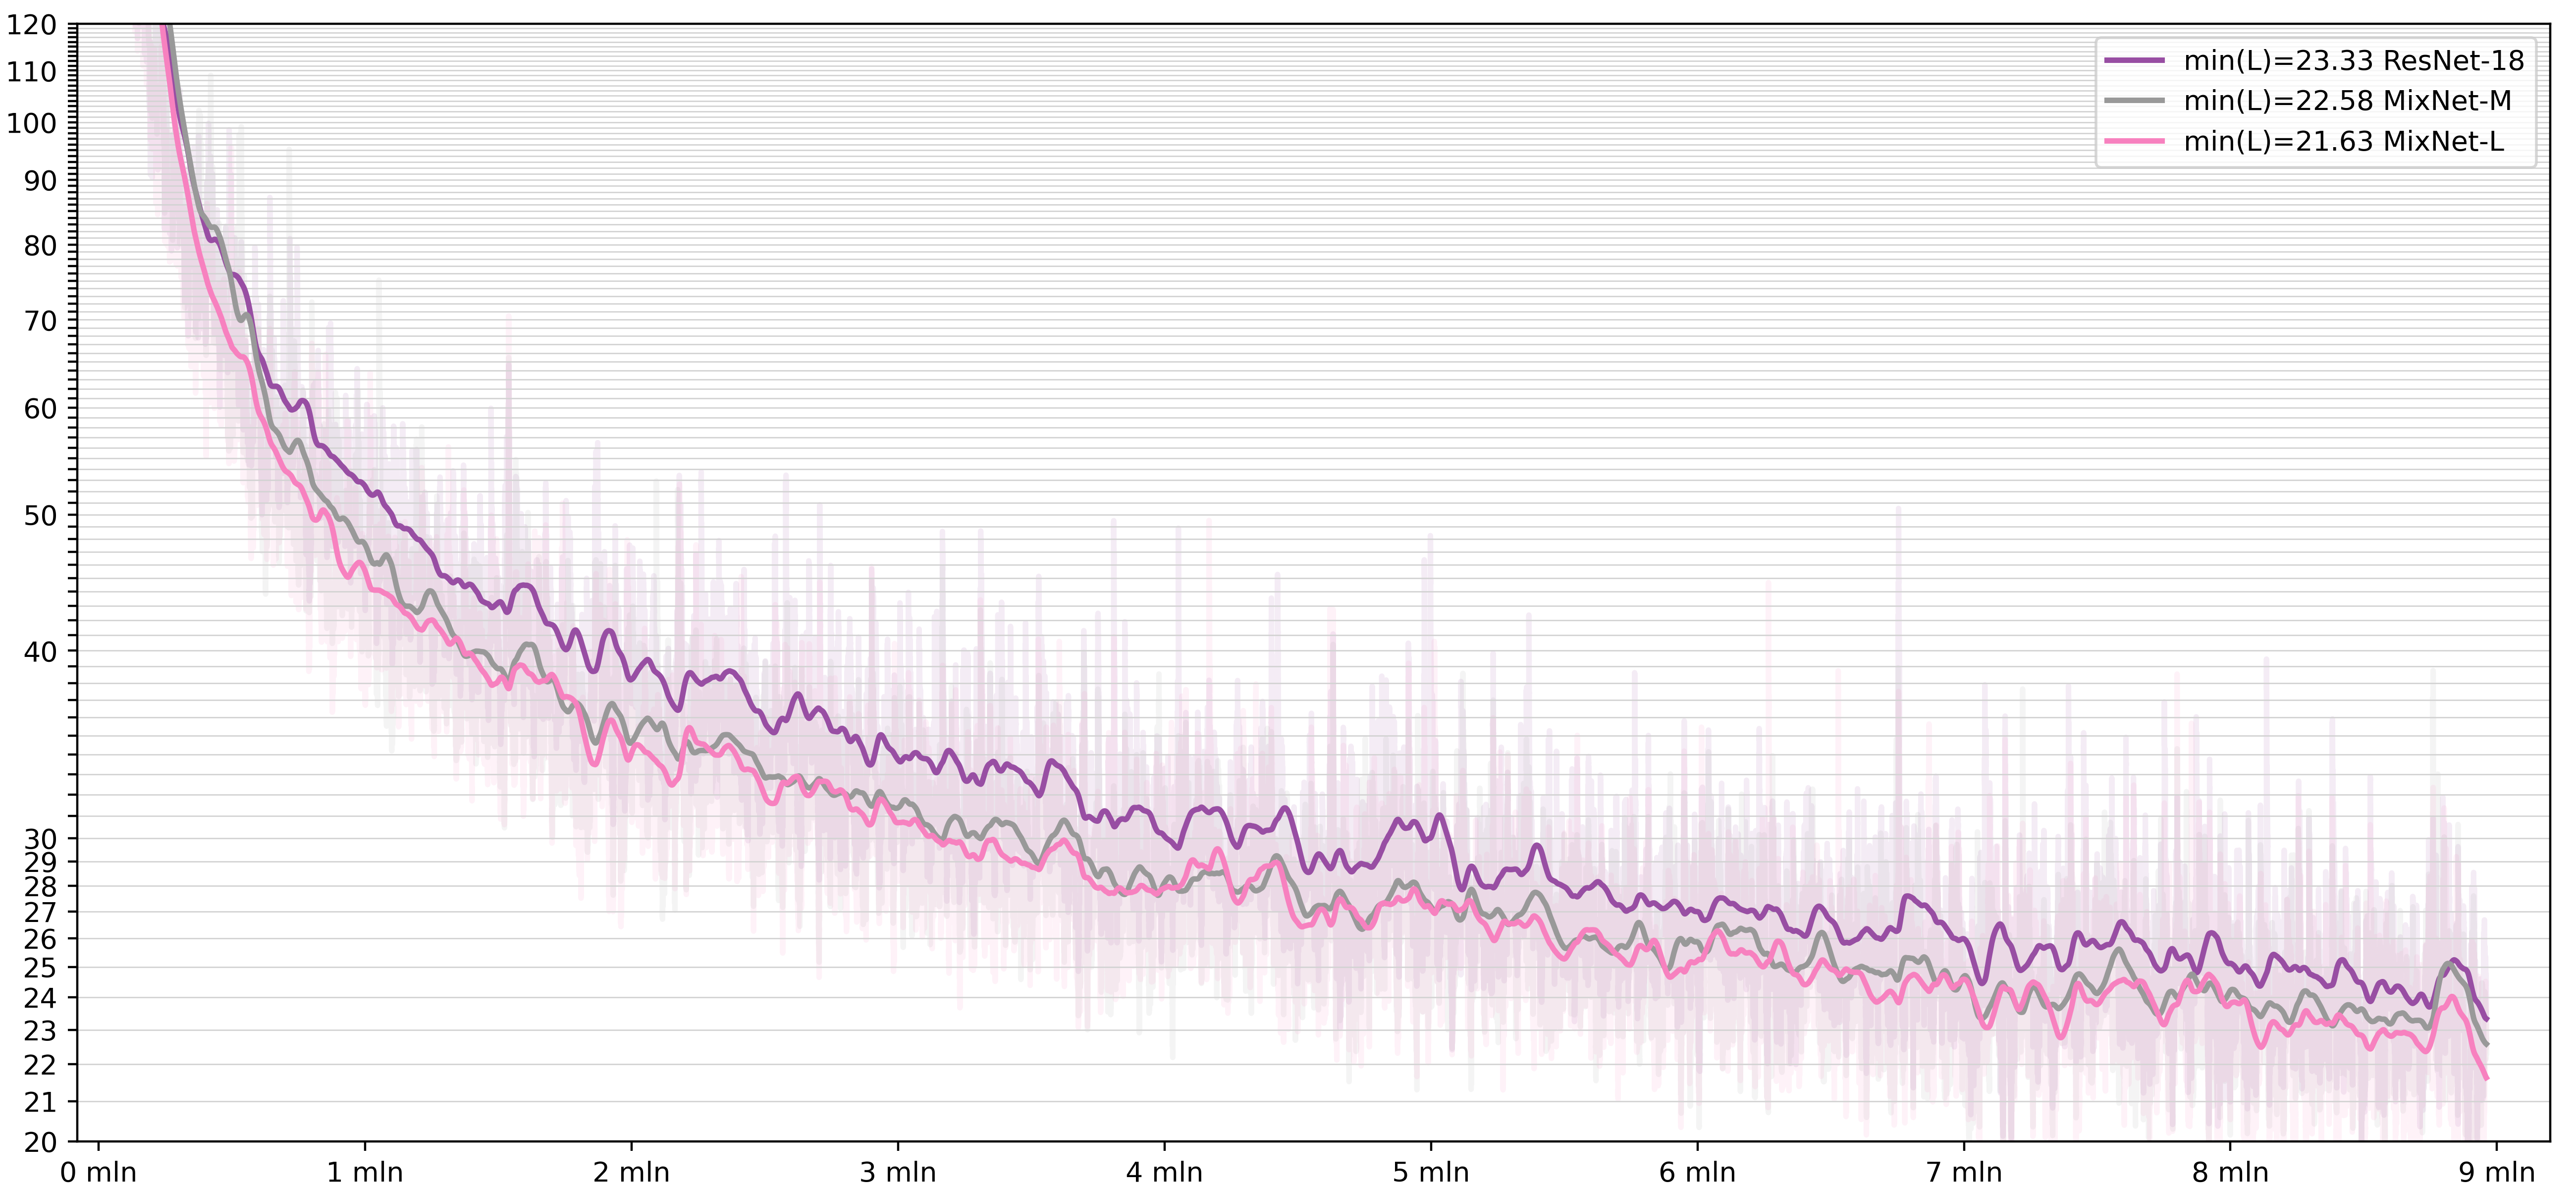
\includegraphics[width=\linewidth]{loss_centerlines_train.png}
    \caption{Wartości funkcji $L$ dla próbek ze zbioru \textbf{treningowego} (wartości najmniejsze podane są dla krzywych uzyskanych z wygładzenia wykładniczego wartości funkcji $L$)}
    \vspace*{1cm}
    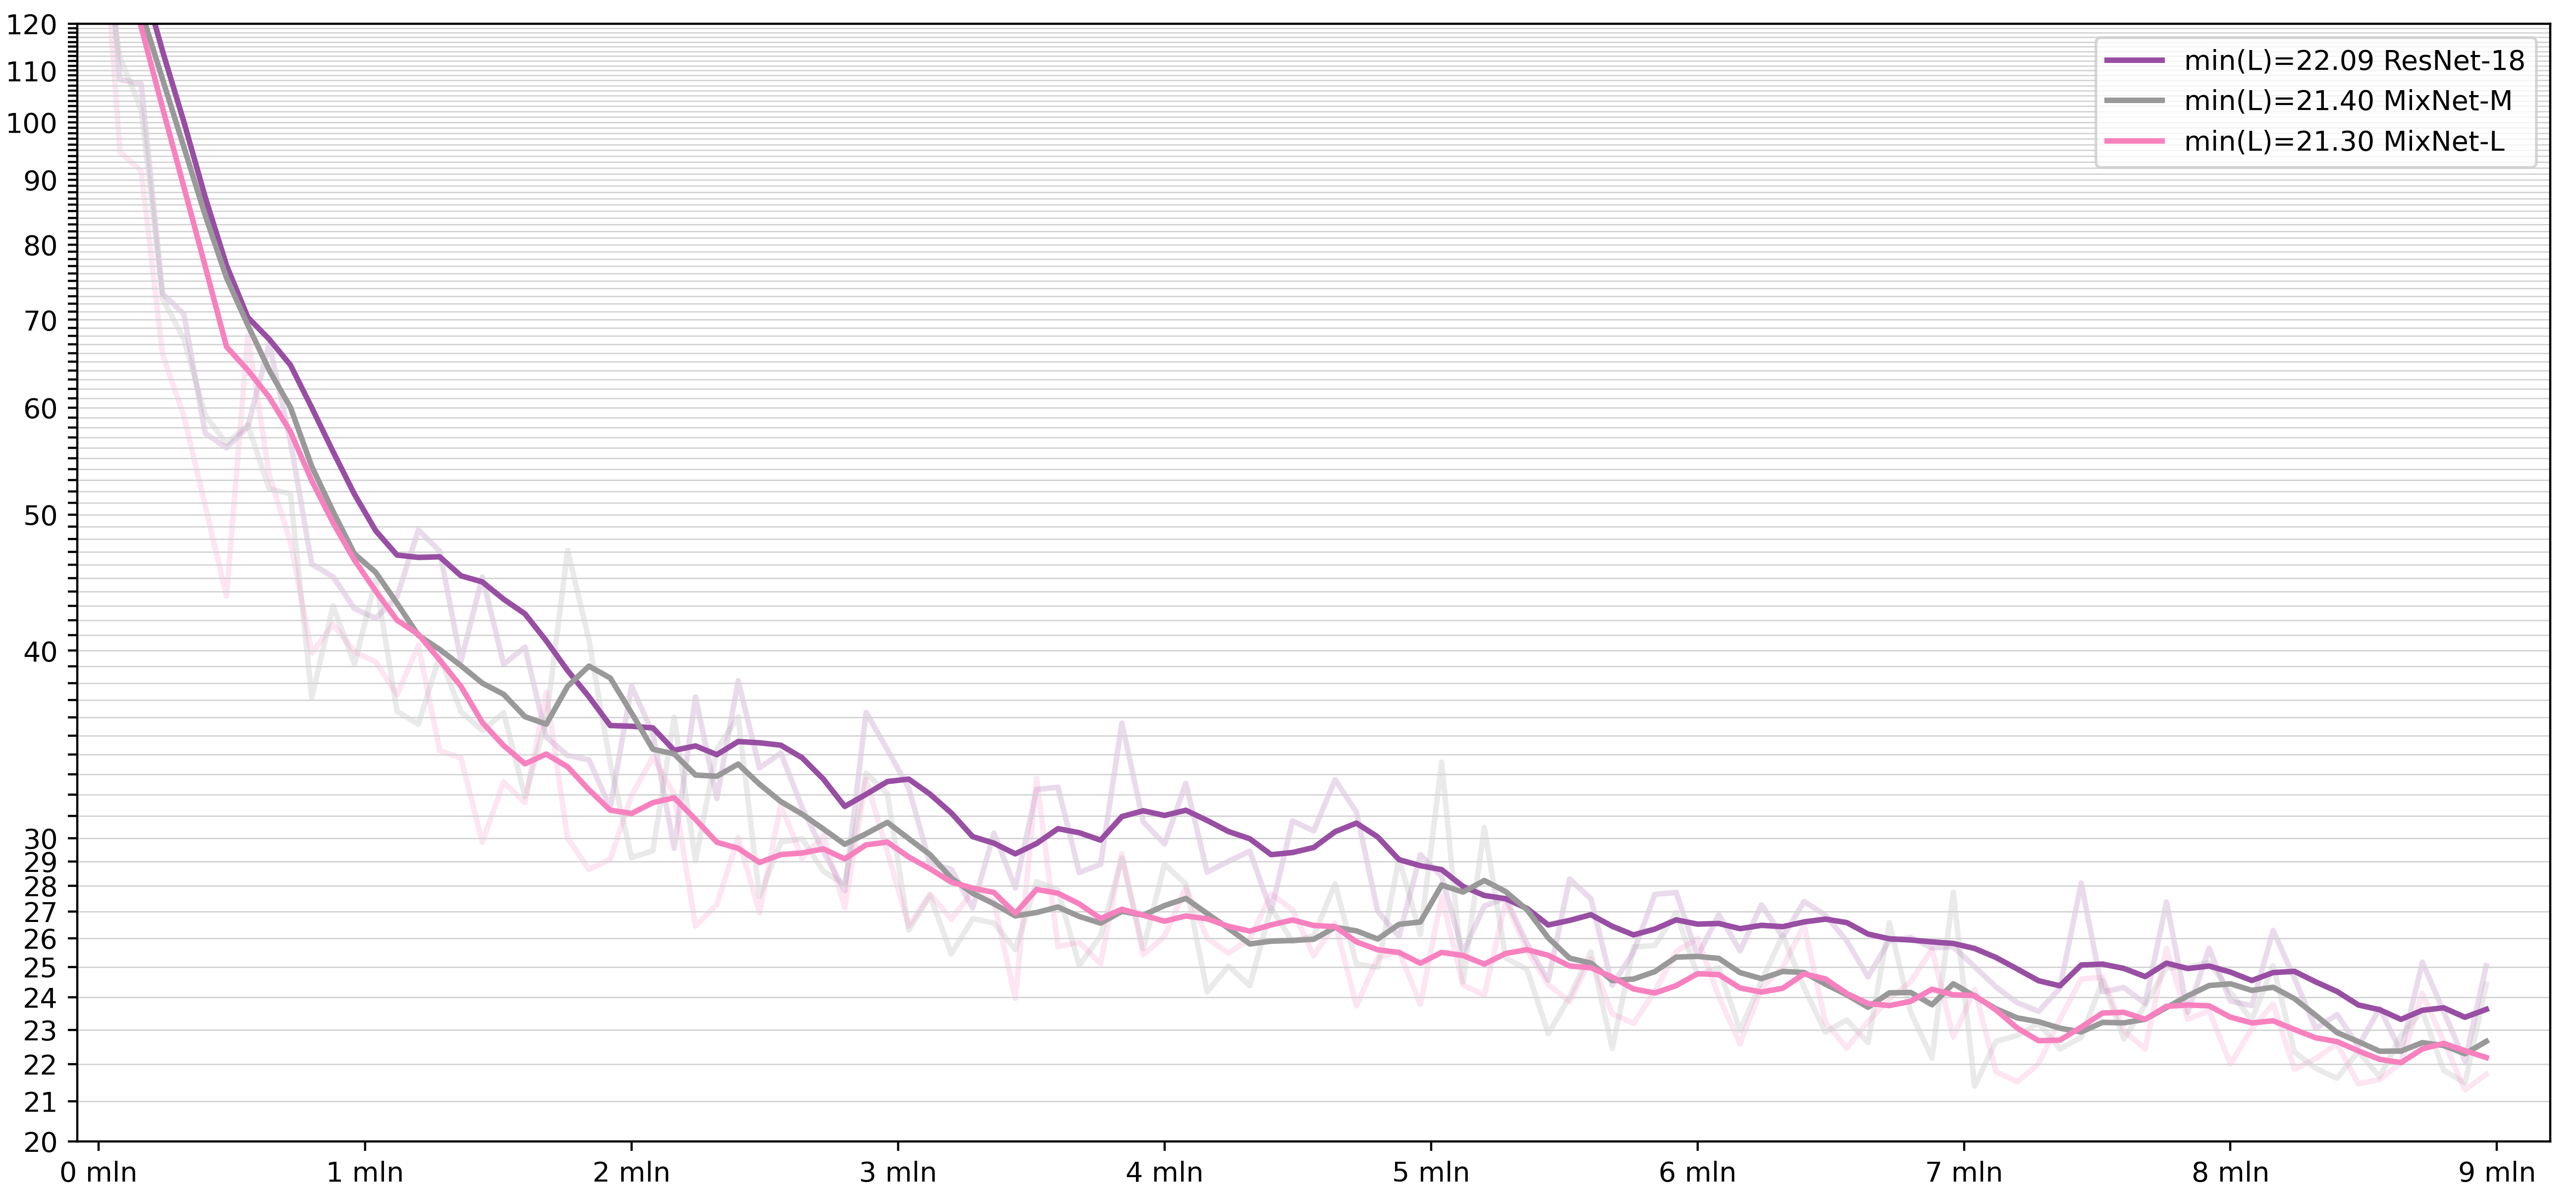
\includegraphics[width=\linewidth]{loss_centerlines_val.png}
    \caption{Wartości funkcji $L$ dla próbek ze zbioru \textbf{walidacyjnego} (wartości najmniejsze podane są dla dokładnych wartości funkcji $L$)}
\end{figure}

\newpage

\section{Opis wizualizacji i wyników}

\subsection{Pierwszy etap}

W pierwszym etapie trenowania, uruchomiono proces dla wszystkich ośmiu sieci neuronowych. Wykonanie jednego cyklu trenowania na pakiecie 16 elementów (ang. batch), zajmowało około 2.18 sekundy. Było to stanowczo za długo, aby przeprowadzić proces trenowania w pełnym zakresie na wszystkich ośmiu sieciach neuronowych. Należy zaznaczyć, że do tak wysokiego czasu cyklu przyczyniły się głównie sieci o dużej liczbie parametrów. Po 465 tys. pakietów (7.44 mln elementów zbioru treningowego), które zostały użyte w procesie trenowania trwającym 12 dni, należało wybrać sieci neuronowe, których trenowanie będzie kontynuowane.

\subsection{Drugi etap}

Wybrano trzy sieci mające najniższe wartości wygładzonej funkcji kosztu na zbiorze walidacyjnym. Były to sieci z następującym szkieletami: \texttt{ResNet-18}, \texttt{MixNet-M}, \texttt{MixNet-L}. Następnie kontynuowano proces trenowania tych trzech sieci. Czas jednego cyklu trenowania zredukowano do 0.44 sekundy. Ten etap trenowania odbył się z wykorzystaniem 1.975 mln pakietów (31.6 mln elementów zbioru treningowego). Etap ten trwał 10 dni.

\subsection{Trzeci etap}

W trzecim etapie przeprowadzono trenowanie wybranych sieci neuronowych z użyciem rasteryzatora \texttt{CenterLines}. Ze względu na ograniczony czas, w którym możliwe byłoby wytrenowanie sieci neuronowych, eksperymenty w trzecim etapie ograniczono do sieci, które wykazały bardzo dobre wyniki z użyciem rasteryzatora \texttt{SemBoxRasterizer} w etapie drugim. Były to sieci o następujących szkieletach: \texttt{ResNet-18}, \texttt{MixNet-M}, \texttt{MixNet-L}. Jeden cykl trenowania trwał 0.53 sekundy. Trenowanie tych sieci trwało 5 dni i odbyło się z wykorzystaniem 560 tys. pakietów (9 mln elementów zbioru treningowego). Wyniki uzyskane z użyciem rasteryzatora \texttt{CenterLines} okazały się gorsze, niż te uzyskane z użyciem rasteryzatora \texttt{SemBoxRasterizer}. Należy mieć na uwadze, że proces trenowania nie został przeprowadzony w pełni (ze względu na ograniczenia czasowe i sprzętowe), możliwe jest, że funkcje kosztu maleją wolniej (z użyciem tego rasteryzatora), ale finalnie osiągnęłyby wartości niższe, niż te uzyskane z rasteryzatorem \texttt{SemBoxRasterizer}. Niestety, aby się o tym przekonać należałoby trenować te 3 sieci przez kolejne kilkadziesiąt dni (do momentu, w którym funkcje kosztu na zbiorze walidacyjnym zaczęłyby rosnąć).